\section{Assignment 1}

\subsection{3D model creation using Zephyr}

The object chosen for the assignment was a plastic statue of an angel.

\begin{figure}[h]
\centering
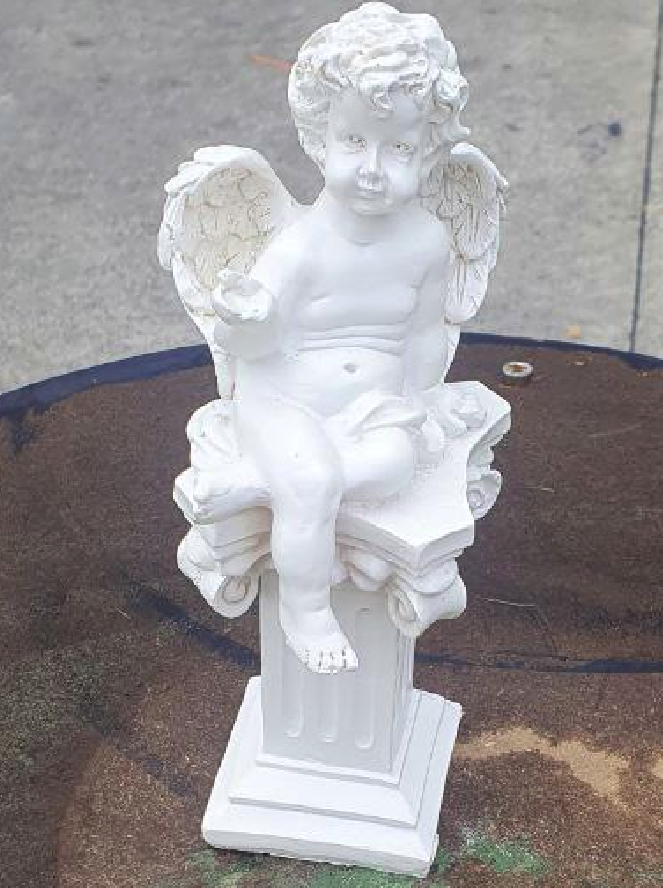
\includegraphics[keepaspectratio,width=0.35\textwidth]{angel}
\end{figure}

119 photos of it were collected, all around it and at three different heights. The 3D model was obtained with Zephyr after the following steps:
\begin{itemize}
\item Sparse point cloud generation, using the 'Human body' and 'High details' presets.
\item Dense point cloud generation, using the 'Human body' and 'High details' presets.
\item Mesh generation, using the 'Default' and 'High details' presets.
\item Textured mesh generation, using the 'Default' and 'High details' presets.
\end{itemize}

\begin{figure}[H]
\centering
\begin{minipage}{0.23\textwidth}
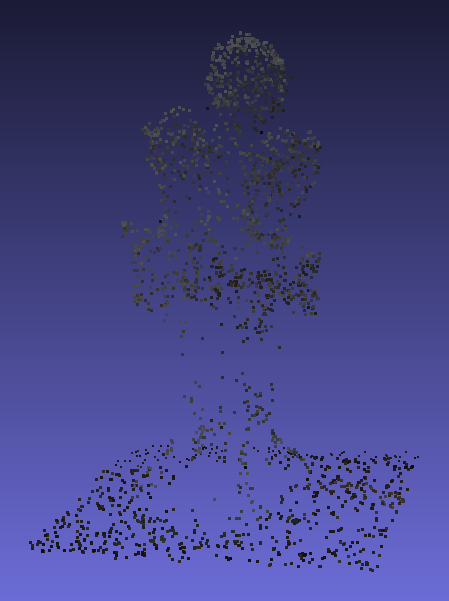
\includegraphics[keepaspectratio,width=0.9\textwidth]{angel_sparse}
\end{minipage}
\begin{minipage}{0.25\textwidth}
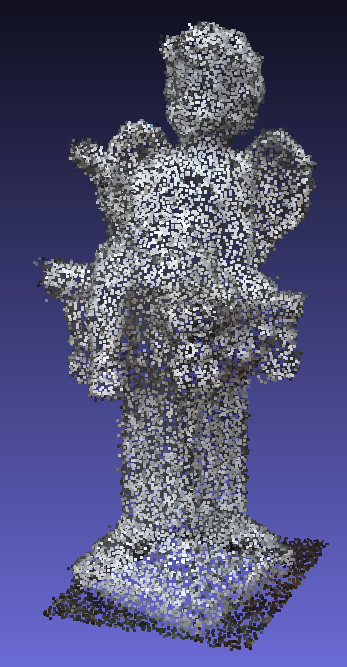
\includegraphics[keepaspectratio,width=0.9\textwidth]{angel_dense}
\end{minipage}
\begin{minipage}{0.25\textwidth}
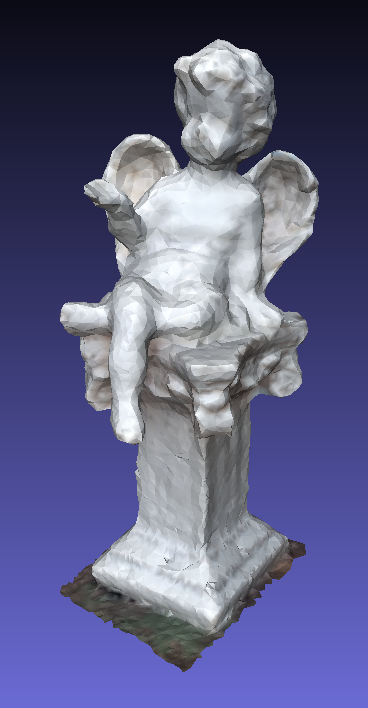
\includegraphics[keepaspectratio,width=0.9\textwidth]{angel_mesh}
\end{minipage}
\begin{minipage}{0.25\textwidth}
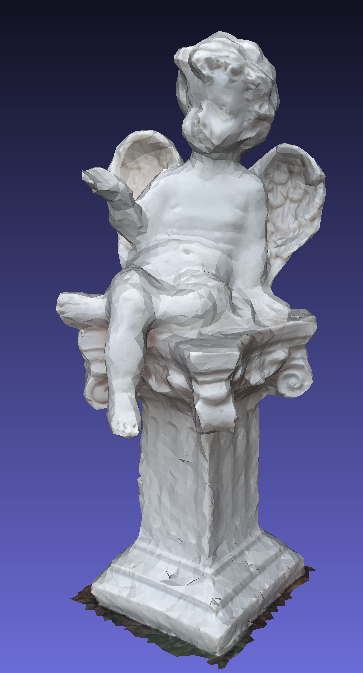
\includegraphics[keepaspectratio,width=0.9\textwidth]{angel_textured_mesh}
\end{minipage}
\caption{From left to right: sparse point cloud, dense point cloud, mesh and textured mesh.}
\end{figure}